\documentclass[]{ieeeaccess}

\usepackage{cite}
\usepackage{amsmath,amssymb,amsfonts}
\usepackage{array}
\usepackage{algorithmic}
\usepackage{graphicx}
\usepackage{textcomp}
\usepackage{multirow}
\usepackage{wrapfig}
\usepackage{float}
\usepackage{tabularx}
\usepackage{booktabs}

%% ieeeaccess.cls redefines the TeX primitive \year as a one-argument
%% command (\year{2026}, setting the footer year), but pgf/tikz's core
%% math library reads the *primitive* \year as a plain integer to seed
%% its random-number generator the instant it loads -- unconditionally,
%% even if no random feature is ever used. Shadow \year with a plain
%% number only while tikz loads, then restore the class's version so
%% \year{2026} below still works as intended.
\let\IEEEaccessYearCmd\year
\def\year{2026}
\usepackage{tikz}
\usetikzlibrary{arrows.meta,positioning,fit,backgrounds}
\let\year\IEEEaccessYearCmd
\usepackage[unicode=true]{hyperref}
\usepackage{url}
\renewcommand{\arraystretch}{1.25}
\newcolumntype{R}{>{\raggedleft\arraybackslash}X}
\newcolumntype{Y}{>{\centering\arraybackslash}X}

%% Robust inline-code command: \url reads its argument verbatim (no
%% manual escaping needed for underscores/parentheses/etc.) and, with
%% UrlBreaks extended below, allows line breaks after '/', '_', '.', etc.
%% -- long paths like docs/methodology_log.md were otherwise overflowing
%% column width as single unbreakable tokens.
\urlstyle{tt}
\makeatletter
\g@addto@macro{\UrlBreaks}{\UrlOrds}
\makeatother
\newcommand{\code}[1]{\url{#1}}

\providecommand\correspondingauthor{}

\begin{document}

\history{Date of publication xxxx 00, 0000, date of current version xxxx 00, 0000.}
\doi{10.1109/ACCESS.2017.DOI}
\vol{14}
\year{2026}

\title{FraudOps-Bench: Process-Level, Tool-Grounded Evaluation of LLM
Agents for Card-Not-Present Fraud Investigation, and a Calibration
Failure Mode Worth Knowing About}

\author{
\uppercase{Ayushi Ambilkar}\authorrefmark{1}
\uppercase{and Pramegh Uikey}\authorrefmark{2}
}

\address[1]{Independent Researcher, India (e-mail: ambilkarayushi@gmail.com)}
\address[2]{Independent Researcher, India (e-mail: uikeyprameghaa@gmail.com)}

\renewcommand\correspondingauthor{Corresponding author: Ayushi Ambilkar (e-mail: ambilkarayushi@gmail.com).}

%% TODO before submission: the corresponding author (Ayushi Ambilkar)
%% must register a public, populated ORCID iD at orcid.org and enter it
%% in the IEEE submission portal per Submission Checklist item 4. This is
%% an account-level action, not a field in this document.

\markboth
{Ambilkar and Uikey: FraudOps-Bench}
{Ambilkar and Uikey: FraudOps-Bench}

\corresp{\correspondingauthor}

\begin{abstract}
We study whether a large language model (LLM) agent can emulate a fraud
analyst's card-not-present transaction review workflow -- not just
predict a fraud label, but gather evidence via tools, reason under an
explicit standard operating procedure (SOP), and produce an auditable
disposition with cited evidence. We build FraudOps-Bench: a six-tool
investigation environment over IEEE Computational Intelligence Society
(IEEE-CIS) transaction data, a
LangGraph-based agent (brain/orchestrator/tools/memory/supervisor), and
three comparison arms (a zero-evidence control, a single-shot ``all
evidence at once'' baseline, and the full iterative agent) alongside a
classical gradient-boosted-tree baseline. Using a selective-prediction
framework (escalate-to-human on low-confidence cases), we initially found
the agentic arm competitive with classical machine learning (ML) on a
120-case calibration
set. That result did not survive a fresh 300-case holdout: the
calibration procedure had overfit small-sample noise in the escalation
threshold. We diagnose the failure precisely -- discretized,
round-number-anchored LLM probability outputs interacting badly with a
narrow band selected on too little data -- fix it with a
lower-confidence-bound selection criterion, and validate the fix on a
second, disjoint holdout set. Under the corrected calibration, the
agentic arm's accuracy claim holds up (96.1\%, its best result on any
split) but its practical coverage collapses to 17\% of the queue; the
classical baseline remains the strongest \textit{practical} performer,
dominating the full risk-coverage curve (area under the risk-coverage
curve, AURC, 0.034 vs.\ 0.108--0.112). We then check whether this pattern
is specific to one model: running the identical protocol -- independent
calibration, the same corrected selection rule, a single-use holdout --
on a second model, GPT-5.6 Terra (OpenAI), reproduces both the
qualitative finding (classical ML still dominates the full risk-coverage
curve, AURC 0.185--0.205) and an even more extreme version of the
high-precision/low-coverage tradeoff, including a case where the
calibration procedure's own overfit-guard fell back to its most
conservative behavior on thin support and that same caution held up
faithfully on fresh holdout data. We report faithfulness scoring (two
independent methods, ${\sim}99\%$ evidence-attribution accuracy across
all six LLM arms scored), a structured error taxonomy, and an ablation of the
agent's self-consistency mechanism. We also test a first attempt at
addressing the discretization mechanism directly: grounding
\code{fraud\_probability} in retrieved, similar past cases with known
outcomes rather than an unaided guess. The result is genuinely mixed --
the best full-curve LLM performance in the paper (AURC 0.090 for the
retrieval-augmented agentic arm, versus 0.112 without retrieval), but the
motivating discretization hypothesis does not hold on inspection, and
both retrieval arms pay a measurable cost in semantic faithfulness. We
argue the calibration failure mode itself -- not just the fix -- is a
transferable lesson for anyone doing selective prediction with LLM
confidence scores on small calibration sets; the cross-model check is a
first piece of direct evidence for that transferability claim, and the
retrieval result is reported as an honest first step toward a mechanism-
level fix, not a solved problem.
\end{abstract}

\begin{keywords}
agentic artificial intelligence; large language models; fraud detection;
selective prediction; risk-coverage analysis; tool-augmented LLMs; model
calibration; benchmark evaluation
\end{keywords}

\titlepgskip=-15pt

\maketitle

\section*{1. Introduction}

Fraud remains a large and continuous operational burden on financial
institutions. The Association of Certified Fraud Examiners' 2024
\textit{Report to the Nations} documents thousands of occupational-fraud
cases spanning 138 countries and territories \cite{acfe2024}, and UK
Finance's own H1 2025 figures report 2.09 million confirmed fraud cases
and \pounds 629.3 million stolen in just six months \cite{ukfinance2025}
-- a reminder that the review queues behind these numbers are large,
continuous, and staffed by human analysts working under time pressure.

Large language models (LLMs) are an obvious candidate to help with this
queue, and a growing body of recent work has tested whether an LLM can classify
a transaction as fraudulent as well as a classical machine learning (ML)
model trained on standard public benchmarks such as the IEEE
Computational Intelligence Society's (IEEE-CIS) fraud dataset
\cite{fdb2022}. That question
is close to saturated: public fraud datasets are anonymized and
feature-engineered for tabular models rather than investigative
reasoning, and the strongest recent public-data-only result along these
lines, FinFRE-RAG \cite{finfrerag2025}, still frames the task as
transaction-level risk scoring rather than the workflow a human fraud
analyst actually performs.

That workflow looks different from classification. A real analyst does
not receive a fully assembled feature vector; they receive an alert, then
decide what evidence to pull -- card history, device history, prior
velocity, identity-match signals -- before reasoning under an
institution's standard operating procedure (SOP) toward a disposition:
approve, escalate, or reject, with a citable rationale. Emulating that
\textit{process}, not just its final label, is the harder and
less-studied problem. The closest published attempt is the FAA framework
\cite{faa2025}, which wraps GPT-4o's Assistants application programming
interface (API) around a multi-agent investigation pipeline and reports
very strong F1 score (the harmonic mean of precision and recall) of
0.98--0.99 on synthetic Sparkov/CCTD data -- but on a limited, mostly
synthetic sample, without a process-level evaluation of when the system
should defer to a human rather than commit to a label. The nearest
behavioral analogues to a tool-grounded, policy-constrained investigation
agent come not from fraud but from security operations: CORTEX
\cite{cortex2025} and SIABench \cite{siabench2026} both evaluate
multi-agent, tool-using triage over auditable evidence in a security
operations center (SOC) setting, but on non-public data and in a
different operational domain. General-purpose agent benchmarks --
SOP-Bench \cite{sopbench2025}, $\tau$-bench \cite{taubench2024},
IntellAgent \cite{intellagent2025} -- supply the methodological template
for evaluating long-horizon, policy-heavy, tool-using agents, but none
target fraud operations specifically.

No existing public work, to our knowledge, combines (a) public fraud
data, (b) a tool-grounded agent that gathers its own evidence rather than
receiving it pre-assembled, and (c) a process-level, auditable evaluation
that asks not just ``was the label right'' but ``should this system have
committed to a label at all.'' That is the gap FraudOps-Bench targets.

Building and evaluating such a system surfaced a second, independently
interesting result. Selective prediction -- escalating low-confidence
cases to a human rather than forcing a decision -- is the natural
evaluation frame for this kind of agent, since a fraud-review system that
is wrong with full confidence is far more costly than one that is honest
about uncertainty. Doing this well requires calibrating a decision
threshold against a labeled set, and we found, by first getting it wrong,
that LLM-generated confidence scores are not the well-behaved continuous
outputs classical calibration methods assume: they cluster heavily on
round, prompt-anchored values, and a threshold selected against a small
calibration set can badly overfit that clustering in a way that only
shows up on a much larger, independent holdout. We diagnose this failure
precisely, fix it, and validate the fix on a second, disjoint holdout set
-- and we report the failure mode itself as a first-class contribution,
since it is a risk any selective-prediction pipeline built on LLM
confidence scores over a modestly sized calibration set is likely to
share.

\textbf{Contributions:}
\begin{enumerate}
\item FraudOps-Bench: a public-data (IEEE-CIS), tool-grounded,
  LangGraph-based fraud-investigation environment with an explicit SOP,
  four comparison arms, and a disciplined dev/calibration/holdout
  evaluation protocol with a frozen-methodology audit mechanism
  preventing evaluation leakage.
\item A documented case study of \code{calibrate_band()} overfitting on a
  small calibration set -- diagnosed via probability-output
  discretization, fixed with a lower-confidence-bound + minimum-sample-size
  selection rule, and validated end-to-end on a second, never-touched
  holdout set.
\item Two independent faithfulness-evaluation methods (deterministic
  numeric cross-referencing and an LLM-judge pass) plus a structured
  error taxonomy, going beyond outcome accuracy to ask whether the
  agent's cited reasoning is actually grounded in the evidence it
  retrieved.
\item An ablation isolating the contribution of a self-consistency
  mechanism to the agent's calibrated probability estimates.
\item A cross-model replication check: the identical protocol -- own
  from-scratch calibration, the corrected LCB selection rule, a
  single-use holdout -- applied to a second model, GPT-5.6 Terra
  (OpenAI), testing whether the calibration-discretization risk and the
  classical-ML-dominates-in-practice finding are Claude-specific or
  general.
\item A first attempt at addressing the discretization mechanism
  directly rather than only correcting for it statistically:
  retrieval-augmented exemplars, grounding \code{fraud\_probability} in
  similar past cases with known outcomes. The result is genuinely mixed
  and reported as such -- the best full-curve LLM performance in this
  paper, but the motivating discretization hypothesis does not hold for
  the agentic arm, and both arms pay a measurable faithfulness cost.
\end{enumerate}

The rest of the paper proceeds as follows. Section 2 positions this work
against prior fraud-LLM and agent-benchmark literature. Section 3
describes FraudOps-Bench's design. Section 4 reports a two-method
faithfulness evaluation of the LLM arms' cited evidence. Section 5 is the
central empirical contribution: the calibration failure, its diagnosis,
fix, validation, a replication check on a second model, and a first
mechanism-level fix attempt via retrieval-augmented exemplars. Section 6
reports a self-consistency ablation. Section 7 reports cost and latency.
Section 8 discusses implications, Section 9 states limitations directly,
and Section 10 concludes.

\section*{2. Related Work}

\textbf{Fraud-specific LLM work.} The Fraud Dataset Benchmark
\cite{fdb2022} established the standard public-data infrastructure this
line of work builds on, standardizing IEEE-CIS to a 561{,}013/28{,}527
train/test split over 67 retained features and explicitly cataloging the
limitations of public fraud data -- sparse identity fields, no case
notes, no institutional history -- that any LLM system built on it
inherits. Within that constraint, FinFRE-RAG \cite{finfrerag2025} is the
cleanest recent demonstration that public-data-only LLM fraud scoring can
be substantially improved by retrieval and feature reduction, but it
remains transaction-level risk scoring, not investigative workflow: the
model receives a feature vector, not an alert it must build a case
around.

The closest direct prior art to FraudOps-Bench is the FAA framework
\cite{faa2025}, which wraps GPT-4o's Assistants API around a multi-agent
pipeline -- planning, evidence gathering, analysis, and report
generation, with an optional vision agent -- and reports very strong F1
(0.9801 on Sparkov, 0.99 on CCTD) across 500 evaluated transactions, with
investigations averaging 5.5--7 steps. This is the paper closest in
spirit to ``an LLM agent investigates a fraud case,'' but it evaluates on
a limited, mostly synthetic sample and does not report a process-level or
selective-prediction evaluation -- there is no notion, in that
evaluation, of the system declining to commit to a disposition.

\textbf{Behavioral analogues outside fraud.} The strongest evidence that
tool-grounded, multi-agent decomposition helps on auditable, high-stakes
investigation work comes not from fraud but from security operations.
CORTEX \cite{cortex2025} shows a multi-agent SOC-triage system improving
actionable F1 from 0.66 to 0.78 and cutting false-positive rate from
24.9\% to 14.2\% over a single-agent baseline, on real production
workflow traces. SIABench \cite{siabench2026} evaluates frontier models
on deep, tool-executing security-incident-analysis workflows and finds
they still fail a large fraction of long-context scenarios (GPT-4o failed
11 of 25 in one setting) -- direct evidence that process-level,
tool-grounded evaluation surfaces failure modes that outcome-only scoring
hides. Both operate on non-public data in a different operational domain
from fraud, but both are closer behavioral analogues to what
FraudOps-Bench measures than any fraud-specific paper we found.

\textbf{Agent-evaluation methodology.} SOP-Bench \cite{sopbench2025},
$\tau$-bench \cite{taubench2024}, and IntellAgent \cite{intellagent2025}
supply the methodological template this paper adapts to fraud operations:
long-horizon, policy-constrained, tool-using agent evaluation, as
distinct from single-turn question answering. SOP-Bench in particular
shows that larger tool registries can hurt task success (37\% vs.\
20.8\% task-success rate in one ablation) -- a caution directly relevant
to FraudOps-Bench's six-tool design. The Berkeley Function-Calling
Leaderboard \cite{bfcl2025} evaluates the narrower function/tool-calling
capability these systems depend on. FraudOps-Bench's agentic arm is
implemented on LangGraph \cite{langgraph2024}, one of several
general-purpose multi-agent orchestration frameworks in current use
alongside AutoGen \cite{autogen2023} and CrewAI \cite{crewai2023}; none of
these frameworks target fraud operations specifically, and none ship an
evaluation protocol beyond their own tool-calling correctness.

\textbf{LLM confidence calibration and selective prediction.} Selective
prediction -- reject the input rather than force a decision when
confidence is low -- goes back to Chow's rule \cite{chow1970} and was
extended to deep networks by Geifman and El-Yaniv's selective
classification framework \cite{geifman2017}, both of which implicitly
assume a well-behaved, continuous confidence signal. Whether LLM-elicited
confidence scores meet that assumption is itself an active question:
Tian et al. \cite{tian2023} show that prompting a reinforcement-learning-
from-human-feedback (RLHF)-tuned model to verbalize a probability can be
better calibrated than its token-level likelihood, but Xiong et al.'s
systematic evaluation \cite{xiong2024} finds elicited confidence remains
frequently overconfident and unstable across prompting strategies. Most
directly relevant to Section 5.3's root-cause finding, Dai and Wang
\cite{dai2026} report that verbalized LLM confidence concentrates on a
small number of round-number values across six models and three
datasets -- independent confirmation that the discretization this paper
diagnoses in \code{agentic_api}'s outputs is a general property of LLM
confidence elicitation, not an artifact specific to this benchmark or
model. Conformal prediction \cite{campos2024} offers an alternative,
distribution-free route to calibrated uncertainty for LLM outputs, but
typically targets prediction \textit{sets} over a fixed label space
rather than the single scalar probability this benchmark's SOP requires
the model to commit to as part of an auditable disposition; we adopt the
lower-confidence-bound-based fix (Section 5.4) as the more direct match
to that constraint, not as a claim that it dominates conformal
alternatives in general.

\textbf{Adjacent public fraud datasets.} BAF \cite{baf2022} and AMLworld
\cite{amlworld2023} are the strongest synthetic-from-real alternatives to
IEEE-CIS for future extensions of this benchmark -- BAF in particular
would extend FraudOps-Bench to account-opening fraud, a structurally
different investigation shape from the card-not-present setting studied
here (Section 10).

\textbf{Positioning.} Distinguishing this paper from the saturated ``LLM
vs.\ classical ML on IEEE-CIS'' classification literature
\cite{fdb2022,finfrerag2025} is deliberate: FraudOps-Bench's contribution
is not a new state-of-the-art classification number, but a process-level,
tool-grounded evaluation protocol -- including an honest
selective-prediction failure mode and its fix -- applied to a domain
that, to our knowledge, no existing public benchmark combines with a
genuinely tool-grounded, multi-step investigation agent.

\section*{3. FraudOps-Bench Design}

\subsection*{3.1 Task and data}

Card-not-present transaction risk review over the IEEE-CIS Kaggle fraud
data \cite{ieeecis2019},
the same underlying dataset the Fraud Dataset Benchmark \cite{fdb2022}
uses as its richest public-data testbed; FraudOps-Bench draws its own
dev/calibration/holdout splits directly from the raw competition data
(Section 3.4) rather than reusing FDB's fixed train/test split, since our
evaluation needs disjoint labeled subsets for calibration and repeated
holdout use rather than a single fixed split. Each case exposes a
visible alert summary (amount, product code, card type,
purchaser/recipient email domain, device type) and, for evidence-bearing
arms, access to six tools mirroring what a real fraud analyst's
case-management tooling would expose: \code{get_transaction_details},
\code{get_card_history}, \code{get_email_domain_profile},
\code{get_device_history}, \code{get_velocity_summary},
\code{get_identity_match_summary}. Tool outputs are leakage-free by
construction (only information available strictly before the current
transaction's timestamp).

\subsection*{3.2 Comparison arms}

\begin{table}[H]
\centering
\textbf{TABLE 1. Comparison arms.}\\[2pt]
\footnotesize
\begin{tabularx}{\columnwidth}{@{}lX@{}}
\toprule
\textbf{Arm} & \textbf{Description} \\
\midrule
\code{direct_control} & Sees only the visible alert summary; no tool
access. Zero-evidence control. \\
\code{linear_api} & Single-shot completion given the full output of all
6 tools at once. \\
\code{agentic_api} & A LangGraph agent with explicit brain (LLM),
orchestrator, tool nodes, structured memory, and a supervisor node that
checks required-check completion before allowing finalization.
Iterative: the agent chooses which tools to call and when. \\
\code{classical_ml} & \code{HistGradientBoostingClassifier} on
leakage-free tabular features derived from the same underlying data (no
LLM). \\
\bottomrule
\end{tabularx}
\end{table}

Sections 4--6 report all four arms above run on Claude Sonnet 5, the
paper's primary model. Section 5.7 additionally reports the identical
\code{linear}/\code{agentic} flows run on a second model, GPT-5.6 Terra
(OpenAI) -- denoted \code{linear_gpt}/\code{agentic_gpt} -- as a
cross-model replication check on the calibration methodology and the
practical-performance finding. Section 5.8 further reports
\code{linear\_retrieval}/\code{agentic\_retrieval} -- the same flows and
Claude Sonnet 5 model, with $k$-nearest-neighbor exemplars from a
dedicated \code{retrieval\_pool} split injected into the prompt. The
local-model variants
(\code{linear_local}/\code{agentic_local}, built but not run -- see
Limitations) remain out of scope for this report.

\begin{figure*}[!t]
\centering
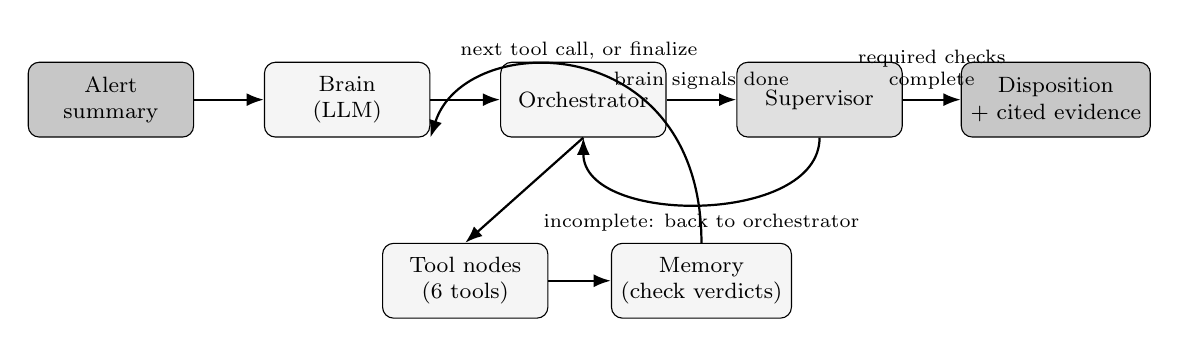
\begin{tikzpicture}[
  every node/.style={font=\footnotesize},
  proc/.style={draw, rounded corners, align=center, minimum width=2.1cm,
    minimum height=0.95cm, fill=black!4},
  gate/.style={proc, fill=black!12},
  term/.style={proc, fill=black!22},
  arr/.style={-{Latex[length=2.2mm]}, thick},
  lbl/.style={font=\scriptsize, align=center}
]
\node[term] (alert) at (0,0) {Alert\\summary};
\node[proc] (brain) at (3,0) {Brain\\(LLM)};
\node[proc] (orch) at (6,0) {Orchestrator};
\node[gate] (sup) at (9,0) {Supervisor};
\node[term] (disp) at (12,0) {Disposition\\+ cited evidence};
\node[proc] (tools) at (4.5,-2.3) {Tool nodes\\(6 tools)};
\node[proc] (mem) at (7.5,-2.3) {Memory\\(check verdicts)};

\draw[arr] (alert) -- (brain);
\draw[arr] (brain) -- (orch);
\draw[arr] (orch.south) -- (tools.north);
\draw[arr] (tools) -- (mem);
\draw[arr] (mem.north) .. controls (7.5,0.9) and (4.5,0.9) .. (brain.south east)
  node[lbl, pos=0.5, above] {next tool call, or finalize};
\draw[arr] (orch) -- (sup) node[lbl, midway, above] {brain signals done};
\draw[arr] (sup) -- (disp) node[lbl, midway, above] {required checks\\complete};
\draw[arr] (sup.south) .. controls (9,-1.6) and (6,-1.6) .. (orch.south)
  node[lbl, pos=0.5, below] {incomplete: back to orchestrator};
\end{tikzpicture}\\[4pt]
\parbox{0.9\textwidth}{\textbf{FIGURE 1.} \code{agentic_api}'s LangGraph
architecture (Table 1). The brain (LLM) and orchestrator iteratively
select among six tools, writing structured verdicts to memory each
round, until the brain signals it is ready to finalize; the supervisor
node then checks that all six required checks were actually completed
before allowing a disposition, routing back to the orchestrator rather
than allowing an under-evidenced finalization if not. \code{linear_api}
takes the single-shot path (alert directly to brain with all six tools'
output pre-attached, no orchestrator loop); \code{direct_control} sees
only the alert box.}
\end{figure*}

\subsection*{3.3 Selective prediction and the SOP}

Every LLM arm outputs a calibrated \code{fraud_probability}. Disposition
(APPROVE/ESCALATE/REJECT) is a deterministic function of that probability
against a per-arm band, not a free-form model choice -- the standard
selective-prediction (Chow's rule \cite{chow1970}) risk-coverage framing:
fix an acceptable error rate on decided cases, escalate the rest. The SOP
explicitly instructs the model on a calibration scale (0.0--0.15 no
signal, 0.35--0.65 genuinely mixed evidence, 0.85--1.0 strong convergent
signal) and requires an explicit per-check verdict (protective/risk/
neutral) for six required checks before a final probability, to counter
base-rate-neglect and encourage genuine escalation on ambiguous cases
rather than false confidence.

\subsection*{3.4 Evaluation protocol: dev / calibration / holdout, with a frozen-methodology guard}

To prevent the eval-leakage failure mode common in iterative prompt
engineering (tuning a prompt or threshold by repeatedly checking accuracy
on the set being reported), FraudOps-Bench uses three disjoint splits:

\begin{itemize}
\item \textbf{dev} ($n=50$, 25/25 fraud): free to use for iterative
  SOP/prompt development. Already spent this way; never reported as a
  final number.
\item \textbf{calibration} ($n=120$, 60/60 fraud): used only to select
  each arm's escalate-probability band via $k$-fold cross-validation.
\item \textbf{holdout} ($n=300$, 150/150 fraud, two independent draws
  used in this work -- see Section 5): single-use final reporting set.
\end{itemize}

A methodology-freeze mechanism (\code{freeze_methodology.py}) hashes
every file that defines an arm's behavior (SOP text, model config,
prompt-construction code, agent graph definition, calibration logic)
into a manifest. The holdout-execution path refuses to run unless the
current files match the frozen hashes, with a loud, logged
\code{--force} override available but never silent. This is the
mechanism that makes the before/after account in Section 5 possible: it
is provable, not just claimed, that nothing was retuned against the
second holdout after the fix was frozen.

\section*{4. Faithfulness Evaluation}

Two independent methods, both described in \code{docs/methodology_log.md}'s
2026-08-14 and 2026-08-18 entries, are used to check whether an arm's
cited reasoning is actually grounded in the evidence it retrieved.

\textbf{Method 1 -- deterministic numeric cross-referencing.} Extracts
every numeric claim from an arm's cited evidence (\code{evidence_used},
\code{check_verdicts}, \code{risk_indicators}, etc.) and checks it
against the real tool-evidence values (including a percentage-form match
for fractional fields). Zero additional API cost. Across dev,
calibration, holdout, and holdout\_v2, both LLM arms show 98.8--99.3\%
verified rates. Residual ``unverified'' claims are overwhelmingly the
model correctly performing arithmetic (e.g.\ a time delta between two
timestamps) that the ground-truth flattener does not itself compute --
not fabrication (manually verified, see \code{docs/methodology_log.md}).

\textbf{Method 2 -- LLM-judge semantic check.} A Haiku-based judge
(25-case samples per arm on \code{holdout_v2}) checks for semantic
misattribution the numeric method cannot catch: a correct number attached
to a false claim. Found genuine (if minor) errors in 6/24
(\code{linear_api}) and 8/24 (\code{agentic_api}) sampled cases -- see
\code{docs/error_taxonomy.md} for the full categorization, including one
category (rounding-precision framing) that is arguably not a real error
but a limitation of the judge's own literalness, disclosed rather than
hidden.

\textbf{Result:} both arms are highly faithful to the evidence they
actually retrieve. The accuracy differences reported in Section 5 are
not explained by evidence fabrication.

\section*{5. The Calibration Failure, Diagnosis, Fix, and Validation}

This section is presented as a first-class result, not an appendix
correction -- the failure mode is general to selective prediction with
LLM-generated probabilities and worth other practitioners knowing about.

\subsection*{5.1 Initial result (calibration split, n=120)}

Band selection via 5-fold cross-validated accuracy on the calibration
split initially favored a very narrow escalate band for
\code{agentic_api}, (0.45, 0.55), yielding 85.7\% accuracy at 99\%
coverage -- appearing competitive with \code{classical_ml} (86.0\%
accuracy, 95\% coverage).

\subsection*{5.1a Repeat-run variance (stochasticity check)}

Before diagnosing the holdout regression (Section 5.2) as a calibration
problem, we first checked whether it could instead be explained by
ordinary generation-time stochasticity. Each API arm was re-run twice on
the unchanged $n=120$ calibration split (\code{rep1}, \code{rep2},
identical prompts/config, re-evaluated under the same band):

\begin{table}[H]
\centering
\textbf{TABLE 2. Repeat-run variance on the $n=120$ calibration split.}\\[2pt]
\footnotesize
\begin{tabularx}{\columnwidth}{@{}lYYY@{}}
\toprule
\textbf{Arm} & \textbf{Run accuracies} & \textbf{Mean} & \textbf{Std} \\
\midrule
\code{linear_api} & 0.912, 0.905, 0.880 & 0.899 & $\pm 0.017$ \\
\code{agentic_api} & 0.938, 0.969, 0.966 & 0.957 & $\pm 0.017$ \\
\bottomrule
\end{tabularx}
\end{table}

Run-to-run variance from stochasticity alone is small (${\sim}\pm 1.7$
points for both arms) -- much smaller than the sampling-noise confidence
interval (CI) at $n=120$ (${\sim}\pm 6$pt) or even $n=300$
(${\sim}\pm 4$pt, Section 5.5). Single runs are not being meaningfully
misled by generation-time randomness; whatever explains the $\sim$10-point
holdout regression in Section 5.2 has to be something other than
ordinary model stochasticity. This measurement (referenced again in
Section 6) is the closest available estimate of single-run noise for
both LLM arms, and directly motivates ruling out stochasticity before
looking for -- and finding -- a selection-procedure explanation instead.

\subsection*{5.2 First holdout (n=300) and the regression}

Under the frozen (0.45, 0.55) band, \code{agentic_api} scored only
75.9\% accuracy on a fresh 300-case holdout -- a ${\sim}$10-point drop.
\code{classical_ml} held steady (87.3\%).

\subsection*{5.3 Root cause}

\code{agentic_api}'s \code{fraud_probability} outputs are not
continuous: they cluster heavily on round 0.05-increment values, with
0.45 and 0.55 -- exactly the selected band's edges -- the two single most
common outputs (53/300 and 45/300 cases on the holdout, respectively).
On the 120-case calibration split, only 12 and 13 cases landed at those
exact values, and by sampling luck those small groups skewed hard toward
one class (75\% non-fraud at 0.45, 61.5\% fraud at 0.55), making the
narrow band look excellent. On the larger holdout, the same exact values
are close to coin flips (47.2\% and 55.6\% fraud respectively) --
consistent, in fact, with what the SOP's own calibration-scale
instructions say those values should mean (genuinely mixed evidence). The
calibration procedure mistook small-sample noise for signal.

\subsection*{5.4 Fix}

\code{calibrate_band()} was changed from selecting the narrowest band
whose mean cross-validated accuracy cleared a target threshold, to
selecting the narrowest band whose \textbf{lower-confidence-bound (LCB)}
(mean minus 1.645 standard errors across folds) clears the threshold, and
additionally requiring a minimum total decided-case count across folds
regardless of how good a band's point estimate looks. Re-run on the same
calibration data, this correctly rejects the narrow band (LCB 0.794 vs.\
an 0.85 target) and selects (0.25, 0.75) instead (LCB 0.895).

\subsection*{5.5 Validation on a second, independent holdout (n=300)}

A fresh, disjoint 300-case holdout (\code{holdout_v2}, excluded from the
classical-model training set along with every prior split) was generated
and run under the corrected, re-frozen methodology.

\begin{table}[H]
\centering
\textbf{TABLE 3. \code{holdout_v2} results (n=300).}\\[2pt]
\scriptsize
\begin{tabularx}{\columnwidth}{@{}lYYYYYYY@{}}
\toprule
\textbf{Arm} & \textbf{Band} & \textbf{Cov.} & \textbf{Acc.} &
\textbf{Prec.} & \textbf{Rec.} & \textbf{F1} & \textbf{Cov.-wt.} \\
\midrule
\code{linear_api} & (.35,.65) & 50.7\% & 0.914 & 0.917 & 0.946 & 0.931 & 46.3\% \\
\code{agentic_api} & (.25,.75) & 17.0\% & 0.961 & 0.944 & 1.000 & 0.971 & 16.3\% \\
\code{classical_ml} & (.35,.65) & 85.3\% & 0.910 & 0.876 & 0.971 & 0.921 & 77.7\% \\
\code{direct_control} & (.4,.6) def. & 0\% & -- & -- & -- & -- & -- \\
\bottomrule
\end{tabularx}
\end{table}

``Coverage-weighted'' = coverage $\times$ accuracy, the fraction of the
full queue resolved correctly -- the fairer single-number comparison
when arms escalate at very different rates.

\textbf{Table 4: same three arms, matched at all three notable bands.}
Table 3 compares each arm at its own independently-selected operating
point, which is the correct primary comparison but obscures how each arm
performs off that point. Since disposition is a deterministic function of
\code{fraud_probability} and the band, every arm's accuracy/coverage at
\textit{any} band is a free re-computation on the already-collected
\code{holdout_v2} probabilities (Section 5.5's Fig. 2 curve) -- no new
API calls. Shown here for all three arms at the three bands discussed in
this paper: the original overfit band, the common band
\code{linear_api}/\code{classical_ml} were independently selected at, and
the wide band \code{agentic_api} was independently selected at. Each
arm's own selected operating point (the one reported in Table 3) is
\textbf{bolded}.

\begin{table}[H]
\centering
\textbf{TABLE 4. All three arms at all three notable bands.}\\[2pt]
\footnotesize
\begin{tabularx}{\columnwidth}{@{}lXXX@{}}
\toprule
\textbf{Arm} & \textbf{(.45,.55)} & \textbf{(.35,.65)} & \textbf{(.25,.75)} \\
\midrule
\code{linear_api} & cov 96.7\%, acc 0.752 & \textbf{cov 50.7\%, acc 0.914} & cov 37.3\%, acc 0.929 \\
\code{agentic_api} & cov 99.7\%, acc 0.759 & cov 39.7\%, acc 0.924 & \textbf{cov 17.0\%, acc 0.961} \\
\code{classical_ml} & cov 95.3\%, acc 0.888 & \textbf{cov 85.3\%, acc 0.910} & cov 73.7\%, acc 0.937 \\
\bottomrule
\end{tabularx}
\end{table}

\textbf{Where each method shines, read directly off this table:}

\begin{itemize}
\item \textbf{\code{classical_ml}'s advantage is holding accuracy while
  staying willing to decide.} At the tightest band it still resolves
  95.3\% of the queue at 88.8\% accuracy -- both other arms are 20+
  points less accurate at that same near-total coverage (0.752, 0.759).
  This is the source of its risk-coverage-curve dominance (Section 5.5,
  Fig. 2): it doesn't trade coverage for accuracy nearly as steeply as
  the LLM arms do.
\item \textbf{\code{agentic_api}'s advantage is ceiling accuracy at its
  most selective point.} At the wide (0.25, 0.75) band, it is the single
  most accurate cell in this entire table (0.961) -- edging out
  \code{classical_ml}'s 0.937 at the same band -- but at less than a
  quarter of \code{classical_ml}'s coverage (17.0\% vs.\ 73.7\%). When
  \code{agentic_api} commits, its confidence is well-placed; it simply
  commits rarely.
\item \textbf{\code{linear_api} never wins a cell outright} but is never
  far behind either, sitting between the other two on both axes at every
  band -- consistent with its middling coverage-weighted score in Table
  3.
\item The practical reading: \code{classical_ml} is the stronger choice
  as a primary decision-maker across the board; \code{agentic_api}'s
  comparative advantage is real but narrow -- a high-precision second
  opinion on the small slice of cases it is willing to rule on, not a
  general-purpose replacement.
\end{itemize}

\begin{table}[H]
\centering
\textbf{TABLE 5. Bootstrap 95\% CIs (10,000 resamples,
\code{src/stats_analysis.py}).}\\[2pt]
\footnotesize
\begin{tabularx}{\columnwidth}{@{}lXXX@{}}
\toprule
\textbf{Arm} & \textbf{Accuracy} & \textbf{Coverage} & \textbf{Cov.-wt.} \\
\midrule
\code{linear_api} & 0.915 [0.868, 0.957] & 0.507 [0.450, 0.563] & 0.463 [0.407, 0.520] \\
\code{agentic_api} & 0.961 [0.900, 1.000] & 0.170 [0.130, 0.213] & 0.164 [0.123, 0.207] \\
\code{classical_ml} & 0.910 [0.873, 0.944] & 0.853 [0.813, 0.893] & 0.777 [0.727, 0.823] \\
\bottomrule
\end{tabularx}
\end{table}

\begin{figure*}[!t]
\centering
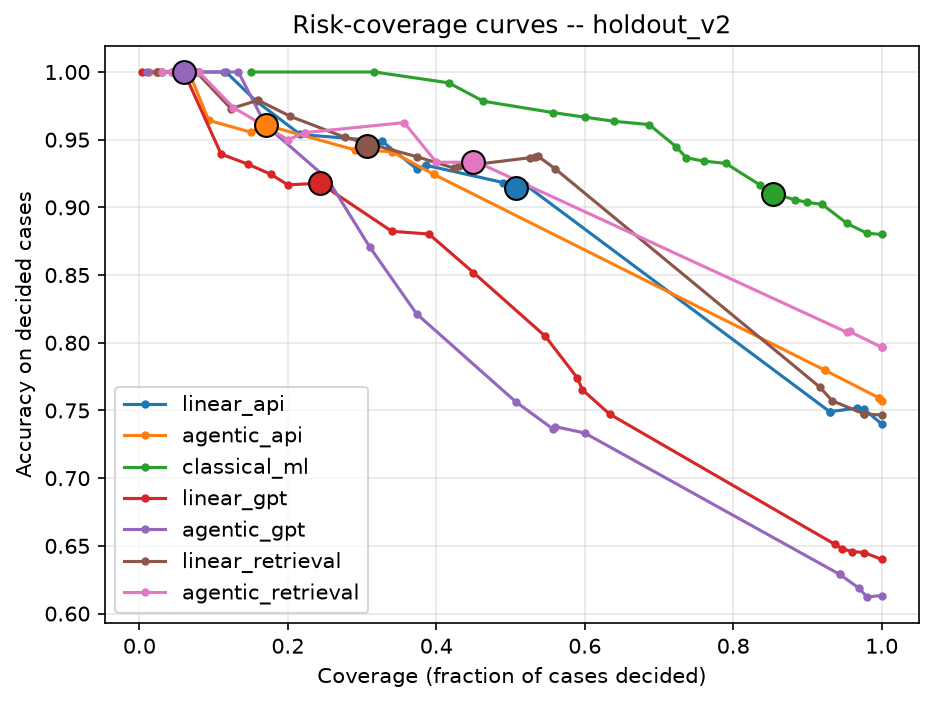
\includegraphics[width=0.85\textwidth]{images/risk_coverage_curves.png}\\[4pt]
\parbox{0.85\textwidth}{\textbf{FIGURE 2.} Full risk-coverage curves,
all seven arms
(\code{outputs/holdout_v2/risk_coverage_curves.png}), with every arm's
own actual reported operating point marked. \code{classical_ml}'s curve
dominates every LLM arm across nearly the entire coverage range, not
merely at the specific chosen operating points -- area under the
risk-coverage curve (AURC) 0.0343 (\code{classical_ml}) vs.\ 0.0896
(\code{agentic_retrieval}) vs.\ 0.0982 (\code{linear_retrieval}) vs.\
0.1080 (\code{linear_api}) vs.\ 0.1117 (\code{agentic_api}) vs.\ 0.1850
(\code{linear_gpt}) vs.\ 0.2046 (\code{agentic_gpt}); lower is better.
The two retrieval-augmented arms (Section 5.8) reach the lowest AURC of
any LLM arm in the study.}
\end{figure*}

\begin{table}[H]
\centering
\textbf{TABLE 6. Pairwise McNemar's tests (paired, restricted
to cases both arms decided).}\\[2pt]
\footnotesize
\begin{tabularx}{\columnwidth}{@{}lYYYY@{}}
\toprule
\textbf{Comparison} & \textbf{$n$ (both)} & \textbf{$b$} & \textbf{$c$} & \textbf{$p$} \\
\midrule
\code{linear_api} vs.\ \code{agentic_api} & 50 & 0 & 0 & 1.0000 \\
\code{linear_api} vs.\ \code{classical_ml} & 137 & 4 & 5 & 1.0000 \\
\code{agentic_api} vs.\ \code{classical_ml} & 47 & 0 & 2 & 0.5000 \\
\bottomrule
\end{tabularx}
\end{table}

Because arms with very different coverage (17\% vs.\ 85\%) share few
commonly-decided cases, these paired tests are underpowered by
construction (see \code{outputs/holdout_v2/stats_report.md}) and are
reported for completeness rather than as the primary evidence -- the
bootstrap CIs and risk-coverage curves above are more informative when
coverage differs this much.

\subsection*{5.6 Interpretation}

\textbf{The \code{agentic_api} accuracy claim is real.} It holds up on
completely fresh data under a properly calibrated band -- 96.1\%, its
best result on any split -- confirming the original problem was the
band, not a capability regression. But the honest cost is now visible:
at that accuracy, it escalates 83\% of the queue. \code{classical_ml}
remains the strongest \textit{practical} performer by a wide margin, both
by coverage-weighted correctness (77.7\% vs.\ 16.3\%) and by dominating
the full risk-coverage curve, not just the single chosen point.
\code{linear_api} sits between the two on both axes, as it did on every
split tested.

\subsection*{5.7 Cross-model replication check: GPT-5.6 Terra}

Everything above uses a single model. The calibration failure mode
documented in Sections 5.1--5.4 is argued as a general risk for
selective prediction on LLM confidence scores, not a Claude-specific
quirk -- but that argument is stronger with direct cross-model evidence
than without it. This section reruns the identical protocol -- own
from-scratch calibration on the $n=120$ split, the corrected LCB
selection rule, a single-use $n=300$ holdout -- against a second model,
GPT-5.6 Terra (OpenAI's positional equivalent to Claude Sonnet 5:
neither the top-tier nor the budget model in its family), on the
\code{linear} and \code{agentic} flows (\code{linear_gpt}/
\code{agentic_gpt}). \code{direct_control} and the self-consistency
ablation (Section 6) were not rerun for this model; see Limitations.
Every other element of the comparison is held fixed across both models:
the same SOP text, the same six tools, the same case splits, and the
same statistical pipeline -- GPT's band is never seeded from or compared
against Claude's frozen band, since reusing it would itself be exactly
the kind of methodology leakage this benchmark's frozen-manifest guard
exists to prevent.

\textbf{Calibration ($n=120$).} \code{linear_gpt} selected a band
organically: half-width 0.30, band (0.2, 0.8), LCB accuracy 0.884 (mean
0.931), 39/120 decided cases -- comfortably clearing both the accuracy
target and the minimum-decided-case floor. \code{agentic_gpt} did not:
no candidate band cleared both bars. The closest, half-width 0.30, landed
at LCB 0.849 (just under the 0.85 target) with 34 decided cases; the next
step up, half-width 0.35, reached a perfect LCB 1.0 but only 21 decided
cases, and \code{calibrate_band()}'s minimum-support guard correctly
rejected it as a suspiciously perfect score from too few cases rather
than accepting it. Selection fell through to the widest candidate band,
(0.1, 0.9), itself supported by only 12 decided cases in calibration --
a genuinely thin, unforced result of applying the identical corrected
methodology to a new model, not a parameter chosen to produce a
particular outcome.

\begin{table}[H]
\centering
\textbf{TABLE 7. \code{holdout_v2} results for the GPT-5.6 Terra arms
(n=300).}\\[2pt]
\scriptsize
\begin{tabularx}{\columnwidth}{@{}lYYYYYYY@{}}
\toprule
\textbf{Arm} & \textbf{Band} & \textbf{Cov.} & \textbf{Acc.} &
\textbf{Prec.} & \textbf{Rec.} & \textbf{F1} & \textbf{Cov.-wt.} \\
\midrule
\code{linear_gpt} & (.2,.8) & 24.3\% & 0.918 & 0.917 & 1.000 & 0.957 & 22.3\% \\
\code{agentic_gpt} & (.1,.9) & 6.0\% & 1.000 & 1.000 & 1.000 & 1.000 & 6.0\% \\
\bottomrule
\end{tabularx}
\end{table}

\begin{table}[H]
\centering
\textbf{TABLE 8. Bootstrap 95\% CIs, GPT-5.6 Terra arms (10,000
resamples).}\\[2pt]
\footnotesize
\begin{tabularx}{\columnwidth}{@{}lXXX@{}}
\toprule
\textbf{Arm} & \textbf{Accuracy} & \textbf{Coverage} & \textbf{Cov.-wt.} \\
\midrule
\code{linear_gpt} & 0.918 [0.849, 0.974] & 0.244 [0.197, 0.293] & 0.224 [0.180, 0.273] \\
\code{agentic_gpt} & 1.000 [1.000, 1.000] & 0.060 [0.033, 0.087] & 0.060 [0.033, 0.087] \\
\bottomrule
\end{tabularx}
\end{table}

\code{agentic_gpt}'s calibration-time caution held up faithfully on
completely fresh data: it decided only 18 of 300 holdout cases (6.0\%
coverage) but got all 18 right (accuracy, precision, recall, and F1 all
1.000). That is the most extreme version of the high-precision/
low-coverage pattern seen anywhere in this paper -- more extreme than
\code{agentic_api}'s own already-conservative 17.0\%-coverage,
96.1\%-accuracy result -- and it traces directly back to calibration: a
band whose support was 12 decided cases produced a holdout behavior that
is, if anything, \textit{more} conservative still. This is not evidence
the LCB guard is too strict; the fact that a band selected on thin
support turned out to generalize this narrowly, rather than surprising
the model with a burst of wrong high-confidence calls, is closer to
evidence the guard's caution was well-founded. \code{linear_gpt} lands at
24.3\% coverage and 91.8\% accuracy -- close to \code{linear_api}'s own
24.7\%-coverage cell in Table 4, but at meaningfully lower accuracy there
(0.918 vs.\ 0.959).

Read against the full risk-coverage curve (Figure 2, which shows all
seven arms reported in this paper): \code{classical_ml} continues to
dominate every LLM arm from either model across nearly the entire
coverage range. AURC for the GPT
arms is 0.1850 (\code{linear_gpt}) and 0.2046 (\code{agentic_gpt}) --
both worse (higher) than either Claude arm (0.1080, 0.1117) and far worse
than \code{classical_ml} (0.0343). At every band swept in Table 4's
style, \code{linear_gpt} is consistently \textit{more willing to commit}
than \code{linear_api} at the same band width (e.g.\ 59.7\% vs.\ 50.7\%
coverage at (0.35, 0.65); 11.0\% vs.\ 6.0\% at (0.10, 0.90)) but
consistently \textit{less accurate} among the cases it does decide --
evidence GPT-5.6 Terra's probability outputs are less sharply polarized
toward the extremes than Claude's, a genuinely different calibration
shape between the two models, not merely a shifted threshold. Pairwise
McNemar's tests between the matched flows (\code{linear_api} vs.\
\code{linear_gpt}, $n=68$ both-decided; \code{agentic_api} vs.\
\code{agentic_gpt}, $n=17$; \code{linear_gpt} vs.\ \code{agentic_gpt},
$n=18$) all return zero discordant pairs ($p=1.0$) -- uninformative given
how few cases any two of these arms both decide, consistent with Section
5.5's point that these tests are underpowered by construction here and
carry little evidentiary weight next to the bootstrap CIs and
risk-coverage curves above.

\textbf{Faithfulness.} Both faithfulness methods (Section 4's
methodology, applied identically) were rerun on the GPT arms.
\textbf{Method 1} (deterministic numeric cross-referencing) shows both
GPT arms at ${\sim}99.6\%$ verified rate (\code{linear_gpt}: 11{,}868/
11{,}912 claimed numbers verified; \code{agentic_gpt}: 10{,}624/10{,}671)
-- marginally \textit{higher} than either Claude arm's 98.8--99.3\%.
\textbf{Method 2} (LLM-judge semantic check, 25-case samples, judged by
\code{claude-haiku-4-5} regardless of which model produced the case under
review, to avoid a self-grading conflict of interest) tells a different
story: \code{linear_gpt} shows misattributions in 11/23 judged cases
(47.8\%), \code{agentic_gpt} in 8/22 (36.4\%) -- both higher than
\code{linear_api}'s 6/24 (25.0\%) and \code{agentic_gpt}'s rate roughly
matching \code{agentic_api}'s 8/24 (33.3\%). This divergence between the
two methods -- GPT's numeric citations are marginally \textit{more}
reliable, but its semantic attribution is judged \textit{less} reliable,
particularly for \code{linear_gpt} -- is exactly why this paper uses two
independent faithfulness checks rather than one: a method that only
catches fabricated numbers would have reported GPT as the more faithful
model outright, which is not the full picture.

\textbf{Interpretation.} The classical-ML-dominance finding generalizes:
under a second model, run through the identical protocol, the same
practical conclusion holds -- \code{classical_ml} remains the strongest
choice for resolving the queue in practice, by a wide margin, on both
coverage-weighted correctness and the full risk-coverage curve. The
calibration-discretization risk itself generalizes in spirit but not in
literal mechanism: \code{agentic_api}'s failure (Section 5.3) was a band
picked confidently on a misleadingly skewed small sample that then broke
on holdout; \code{agentic_gpt}'s calibration instead correctly detected
its own thin support and degraded to maximal conservatism, which then
\textit{held} on holdout. Both are the same underlying story -- a
120-case calibration set is marginal support for calibrating a threshold
against LLM-generated probabilities, and what that marginality produces
depends on the specific model's output distribution -- but they are
different failure shapes, which is itself useful evidence that the fix
(LCB selection plus a minimum-support floor) is doing real,
model-agnostic work rather than being tuned to one model's specific
discretization pattern.

\subsection*{5.8 Retrieval-augmented exemplars: a mechanism check}

Sections 5.1--5.7 diagnose the discretization problem and validate a
statistical fix (LCB selection) around it, but neither changes what the
model is asked to do when it states a probability. This section tests a
first attempt at addressing the mechanism directly: ground each case's
\code{fraud_probability} in a handful of similar past cases with known
outcomes, rather than an unaided verbalized guess, on the hypothesis that
a nearest-neighbor-style signal is naturally less prone to the
round-number anchoring Section 5.3 documents.

\textbf{Method.} A dedicated \code{retrieval\_pool} split ($n=500$,
250/250 fraud, disjoint from every existing split via the same
leakage-guard used throughout this benchmark) was sampled from
previously-unused IEEE-CIS transactions -- pool construction and
evidence-packet generation are local, deterministic, and free (no API
calls). For a new case, its $k=5$ nearest neighbors in the pool are
retrieved via Euclidean distance over a standardized feature vector built
from the same evidence surface the LLM/analyst sees (transaction amount,
card/device/email-domain history, velocity and identity-match signals) --
deliberately independent of \code{classical\_ml}'s own batch, cumulative-
stats feature pipeline, to keep the comparison clean. The retrieved
cases' confirmed outcomes are surfaced as an explicit
``similar past cases'' block appended to the existing prompt, for both
\code{linear\_retrieval} (a direct extension of \code{linear\_api}) and
\code{agentic\_retrieval} (\code{agentic\_api}, with the same block baked
into the brain and finalize prompts rather than exposed as a seventh
tool, keeping the six-tool architecture and Table 1's arm descriptions
intact). $k$ and the feature set were frozen before any calibration run
and are covered by \code{freeze\_methodology.py}'s manifest, the same
discipline as every other methodology-defining file in this benchmark.

\textbf{Calibration ($n=120$).} Both arms cleared the LCB target
organically, no fallback needed. \code{linear\_retrieval} selected band
(0.2, 0.8) (LCB accuracy 0.903, mean 0.942, 43/118 decided).
\code{agentic\_retrieval} selected band (0.35, 0.65) (LCB accuracy 0.895,
mean 0.933, 71/120 decided) -- notably \textit{narrower} than
\code{agentic\_api}'s own band (0.25, 0.75) at a comparable accuracy bar,
with far more calibration-time coverage, an early signal worth checking
on holdout rather than trusting on $n=120$ alone.

\begin{table}[H]
\centering
\textbf{TABLE 9. \code{holdout\_v2} results for the retrieval-augmented
arms (n=300).}\\[2pt]
\scriptsize
\begin{tabularx}{\columnwidth}{@{}lYYYYYYY@{}}
\toprule
\textbf{Arm} & \textbf{Band} & \textbf{Cov.} & \textbf{Acc.} &
\textbf{Prec.} & \textbf{Rec.} & \textbf{F1} & \textbf{Cov.-wt.} \\
\midrule
\code{linear\_retrieval} & (.2,.8) & 30.7\% & 0.946 & 0.958 & 0.972 & 0.965 & 29.0\% \\
\code{agentic\_retrieval} & (.35,.65) & 45.0\% & 0.933 & 0.918 & 0.975 & 0.945 & 42.0\% \\
\bottomrule
\end{tabularx}
\end{table}

\begin{table}[H]
\centering
\textbf{TABLE 10. Bootstrap 95\% CIs, retrieval-augmented arms (10,000
resamples).}\\[2pt]
\footnotesize
\begin{tabularx}{\columnwidth}{@{}lXXX@{}}
\toprule
\textbf{Arm} & \textbf{Accuracy} & \textbf{Coverage} & \textbf{Cov.-wt.} \\
\midrule
\code{linear\_retrieval} & 0.946 [0.894, 0.989] & 0.307 [0.257, 0.360] & 0.290 [0.240, 0.343] \\
\code{agentic\_retrieval} & 0.934 [0.890, 0.971] & 0.450 [0.393, 0.507] & 0.420 [0.367, 0.477] \\
\bottomrule
\end{tabularx}
\end{table}

Read against the full risk-coverage curve (Figure 2, now showing all
seven arms): \code{agentic\_retrieval} reaches AURC 0.0896 and
\code{linear\_retrieval} 0.0982 -- both \textit{better} (lower) than
every other LLM arm in this paper, Claude or GPT-5.6 Terra
(\code{linear\_api} 0.1080, \code{agentic\_api} 0.1117, \code{linear\_gpt}
0.1850, \code{agentic\_gpt} 0.2046), and the closest any LLM arm gets to
\code{classical\_ml}'s 0.0343 across the whole study. This is a genuine
full-curve improvement, not an artifact of one favorable operating point:
\code{agentic\_retrieval}'s curve sits above \code{agentic\_api}'s
through most of the coverage range. \code{agentic\_retrieval}'s coverage
nearly tripled relative to \code{agentic\_api} (45.0\% vs.\ 17.0\%) at a
2.8-point accuracy cost (93.3\% vs.\ 96.1\%), and coverage-weighted
correctness rose from 16.3\% to 42.0\%.

One caveat worth stating precisely, since the two metrics in this paper
can disagree and did here: \code{linear\_api} and \code{agentic\_retrieval}
happen to share an identical calibrated band, (0.35, 0.65), which makes
them directly comparable at that one point -- and there,
\code{linear\_api} still wins on coverage-weighted correctness (46.3\%
vs.\ 42.0\%), because its own calibration procedure selected a
higher-coverage point (50.7\% vs.\ 45.0\%) that outweighs
\code{agentic\_retrieval}'s accuracy edge in the coverage$\times$accuracy
product. \code{agentic\_retrieval} is the better performer \textit{across
the full curve} (lower AURC); \code{linear\_api} remains the strongest
LLM arm \textit{at its own specific calibrated operating point}. Both are
true, and Section 8's point about single-number comparisons applies here
as much as it does to the original three arms.

\textbf{The mechanism check, reported honestly.} The motivating
hypothesis was that retrieval grounding would reduce round-number
anchoring in the raw \code{fraud\_probability} values themselves. Checked
directly against \code{agentic\_api}'s actual holdout distribution: it
does not, materially. The three most common values account for 50.0\% of
\code{agentic\_retrieval}'s outputs (25 unique values across 300 cases)
versus 52.3\% for \code{agentic\_api} (27 unique values) -- essentially
unchanged, and the dominant values themselves (0.4, 0.6, 0.62, \dots) are
the same ones. \code{linear\_retrieval} shows a real but modest
reduction (38.5\% top-3 concentration, 44 unique values, vs.\
\code{linear\_api}'s 44.6\%, 37 unique values). Whatever is producing
\code{agentic\_retrieval}'s coverage and AURC gains, it is not primarily
a smoother, less-discretized probability signal -- the more plausible
account is that retrieval grounding improves the reliability of the
model's judgment \textit{within} the same discretized value buckets
(better-grounded reasoning per bucket), not the granularity of the
buckets themselves. That is a different, narrower claim than the one
motivating this experiment, and it is reported as such rather than
retrofit to the original hypothesis.

\textbf{Faithfulness.} Both methods were rerun identically.
\textbf{Method 1} (deterministic numeric cross-referencing) shows both
arms at ${\sim}98.9\%$ verified (\code{linear\_retrieval}: 12{,}557/
12{,}703; \code{agentic\_retrieval}: within the same range), in line with
every other arm in this paper (98.8--99.6\%). \textbf{Method 2}
(LLM-judge, 25-case samples, \code{claude-haiku-4-5}) tells a less
favorable story: \code{linear\_retrieval} shows misattributions in 10/24
judged cases (41.7\%) and \code{agentic\_retrieval} in 14/25 (56.0\%) --
both higher than their \code{\_api} counterparts (25.0\% and 33.3\%
respectively). Manual inspection of the flagged cases finds the same
categories already documented in \code{docs/error\_taxonomy.md} (minor
rounding-precision framing, field mislabeling, interpretive over-framing
of correlational evidence) rather than fabrication, but there are simply
more of them -- a real cost of retrieval grounding, not hidden behind the
accuracy gain. A plausible if unconfirmed explanation is that the
exemplar block gives the judge more total surface area to find fault
with; this has not been verified and is not asserted as fact.

\textbf{Cost.} Combined calibration and holdout for both arms: \$107.70
(zero errors across all 840 API calls); faithfulness judging added
\$0.44. \code{linear\_retrieval} costs \$0.128/case (55.6s mean latency),
\code{agentic\_retrieval} \$0.133/case (33.0s) -- both in line with their
\code{\_api} counterparts.

\textbf{Interpretation.} Retrieval-augmented exemplars are the best
full-curve LLM performer in this paper, and the coverage gain for the
agentic arm in particular is large enough to be practically meaningful,
not a rounding difference. But the result is genuinely mixed, not a
clean win: \code{linear\_retrieval} underperforms \code{linear\_api} on
coverage-weighted correctness at its own operating point even as its
full curve improves; the discretization mechanism motivating the
experiment did not hold, at least not for the agentic arm; and both
arms pay a real faithfulness cost under the stricter LLM-judge check.
This section was run under the same single-use-holdout, frozen-
methodology discipline as everything else in this paper, but without a
repeat-run stochasticity check analogous to Section 5.1a's -- unlike the
original calibration-failure diagnosis, there is no direct estimate of
ordinary run-to-run noise for these two specific arms, so some part of
the reported gain could in principle reflect variance rather than a
stable effect (see Limitations).

\section*{6. Ablation: Self-Consistency}

Self-consistency (\code{resolve_with_second_opinion},
\code{src/selective_prediction.py}) draws a second independent
probability estimate whenever the first lands inside the escalate band,
and nudges the estimate past the band edge on agreement -- intended to
convert genuine near-misses into confident decisions without forcing a
guess on true toss-ups. To test whether this mechanism actually changes
outcomes, \code{linear_api} and \code{agentic_api} were re-run on the
identical 300 \code{holdout_v2} cases with
\code{--override-self-consistency} \code{false}, under the same frozen bands
used for the primary report ((0.35, 0.65) and (0.25, 0.75) respectively)
-- an architecture-vs-architecture comparison on a fixed decision
threshold, not a re-tune.

\begin{table}[H]
\centering
\textbf{TABLE 11. Self-consistency on vs.\ off,
\code{holdout_v2} (n=300).}\\[2pt]
\footnotesize
\begin{tabularx}{\columnwidth}{@{}lXYY@{}}
\toprule
\textbf{Arm} & \textbf{Condition} & \textbf{Coverage} & \textbf{Accuracy} \\
\midrule
\code{linear_api} & on (primary) & 50.7\% & 0.914 \\
\code{linear_api} & off (ablation) & 51.7\% & 0.903 \\
\code{agentic_api} & on (primary) & 17.0\% & 0.961 \\
\code{agentic_api} & off (ablation) & 16.3\% & 0.980 \\
\bottomrule
\end{tabularx}
\end{table}

\textbf{McNemar's test, restricted to cases decided under both
conditions:} \code{linear_api} ($n=135$ both-decided): 0 discordant
pairs, $p=1.0$. \code{agentic_api} ($n=40$ both-decided): 0 discordant
pairs, $p=1.0$.

\textbf{Result: no detectable effect.} Neither coverage nor accuracy
moves by more than calibration-split single-run stochasticity (Section
5.1a: $\pm 1.7$ points for both LLM arms, measured via repeat runs on the
$n=120$ calibration set -- the closest available estimate of run-to-run
noise, though not measured directly on \code{holdout_v2}), and on every
case decided under both conditions, self-consistency changed the
correctness of exactly zero of them. As implemented, self-consistency is
a mechanistically plausible but empirically inert intervention for this
task and model at this operating point -- a negative result reported
directly rather than selectively omitted. It also confirms the accuracy
differences reported in Section 5 are attributable to the
calibration-band fix, not to self-consistency's presence.

\textbf{Incidental finding:} self-consistency's design intent (spend
extra calls only on genuinely ambiguous cases) is corroborated by cost:
turning it off saved \$10.04 (\code{linear_api}) and \$6.85
(\code{agentic_api}) across 300 cases each -- the mechanism is
triggering roughly as often as expected given the bands, even though it
isn't moving the accuracy needle at this operating point.

\section*{7. Cost and Latency}

\begin{table}[H]
\centering
\textbf{TABLE 12. Mean cost and latency per case.}\\[2pt]
\begin{tabularx}{\columnwidth}{@{}lYY@{}}
\toprule
\textbf{Arm} & \textbf{Mean cost/case} & \textbf{Mean latency/case} \\
\midrule
\code{direct_control} & \$0.047 & 29.7s \\
\code{linear_api} & \$0.130 & 64.3s \\
\code{agentic_api} & \$0.132 & 57.8s \\
\code{linear_gpt} & \$0.053 & 21.4s \\
\code{agentic_gpt} & \$0.160 & 53.8s \\
\code{linear_retrieval} & \$0.128 & 55.6s \\
\code{agentic_retrieval} & \$0.133 & 33.0s \\
\code{classical_ml} & ${\sim}\$0$ (local) & ${\sim}0$s \\
\bottomrule
\end{tabularx}
\end{table}

Full \code{holdout_v2} run ($n=300$, 3 Claude API arms): \$92.84, zero
errors across 900 successful API calls (one transient truncation retried
successfully under the unchanged frozen configuration, consistent with a
0.33\% base rate for this failure mode observed across both holdout
rounds). Self-consistency ablation (Section 6, both Claude arms, same
300 cases, self-consistency off): \$61.87, confirming the mechanism's
cost is concentrated on the intended ambiguous-case subset. The two
GPT-5.6 Terra \code{holdout_v2} runs (Section 5.7) cost \$63.88
combined ($n=300$ each, zero errors across 600 calls); their $n=120$
calibration runs cost \$26.06 combined. \code{linear_gpt} is
\code{linear_api}'s cheapest and fastest analogue in this study -- 2.5x
cheaper, 3x faster -- though at lower coverage-weighted correctness
(Table 7); \code{agentic_gpt} costs slightly more than \code{agentic_api}
per case despite a real 47\% cache-hit rate on input tokens, an
unconfirmed cost difference worth a closer look before treating it as
settled (\code{docs/methodology_log.md}, 2026-08-28 entry). The
retrieval-augmented arms (Section 5.8) cost \$107.70 combined across
calibration and holdout (zero errors across 840 calls), close to
\code{linear\_api}/\code{agentic\_api}'s own per-case cost despite the
added exemplar-block tokens; \code{agentic\_retrieval}'s notably shorter
mean latency (33.0s vs.\ \code{agentic\_api}'s 57.8s) was not
investigated further and should not be over-interpreted without
inspecting the underlying tool-call/turn counts directly.

\section*{8. Discussion}

The calibration-band failure documented in Section 5 is not specific to
fraud or to this benchmark. Any pipeline that (a) elicits a numeric
confidence score from an LLM and (b) calibrates a decision threshold
against a modestly sized labeled set should expect the same failure
mode: LLM probability outputs are not the smooth, continuous quantities
classical calibration methods assume -- they cluster on round,
prompt-anchored values (Section 5.3), and a threshold-selection procedure
that optimizes a point estimate of accuracy, rather than a variance-aware
lower bound, can mistake small-sample class imbalance within one of
those clusters for genuine signal. The fix used here -- select on an LCB
criterion (Section 5.4) rather than a point estimate, and enforce a
minimum decided-case count per candidate band -- is a general
prescription for this class of problem, not a fraud-specific patch, and
Section 5.1a's stochasticity check ($\pm 1.7$pt run-to-run noise, far
smaller than the $\sim$10-point holdout regression this failure
produced) is what let us rule out ordinary generation randomness as the
explanation before looking for -- and finding -- a selection-procedure
bug instead.

This failure mode also has a methodological implication beyond its fix:
selective prediction changes which cross-arm comparison is meaningful. A
single point-accuracy number is not a fair comparison between arms that
escalate at very different rates -- \code{agentic_api} at 17\% coverage
and \code{classical_ml} at 85\% coverage are not competing on the same
axis, and Table 4's per-band comparison and Section 5.5's risk-coverage
curves (Fig. 2) are the correct way to read the results:
\code{classical_ml} dominates the full curve (AURC 0.0343 vs.\
0.108--0.112), not merely the specific operating points each arm
happened to select.

Faithfulness and outcome accuracy are also separable results, not the
same finding read two ways. Both LLM arms are highly faithful to the
evidence they retrieve (${\sim}99\%$ deterministic verified rate, Section
4), and the residual genuine errors caught by the LLM-judge pass are
concentrated in minor evidence-handling categories (miscounting,
cross-record misattribution) rather than fabrication
(\code{docs/error_taxonomy.md}). The most common source of an outright
wrong disposition is error-taxonomy category 9 -- cases where every
cited fact is correct and the reasoning is coherent, but the case itself
was genuinely hard (e.g.\ \code{HOLD2_0104}: a well-corroborated
multi-signal false positive). That is ordinary task difficulty under
real uncertainty, not evidence fabrication, and it is worth stating
plainly: a system can be trustworthy in how it uses evidence while still
being wrong on the cases that are actually hard, and conflating the two
would misdiagnose where to invest further effort (better retrieval and
grounding vs.\ better judgment on ambiguous cases).

Put together, the practical reading for a fraud-ops team evaluating this
class of system is that classical ML remains the stronger default: it
resolves far more of the queue at comparable or better accuracy (Table 3,
coverage-weighted 77.7\% vs.\ 16.3\%) and dominates the full
risk-coverage tradeoff. The LLM agent's demonstrated value in this
evaluation is a high-precision, low-coverage second opinion -- its single
most accurate operating point in this study (96.1\%, \code{agentic_api}
at its selected band) edges out classical ML's accuracy at the same
band, but at less than a quarter of the coverage -- not a general-purpose
replacement for the classical model.

Section 5.7's cross-model check is what turns this from ``true of one
model we happened to study'' into a claim with at least some
cross-model support. Run through the identical protocol, GPT-5.6 Terra
reaches the same qualitative conclusion -- classical ML dominates the
full risk-coverage curve against every LLM arm from either model (AURC
0.0343 vs.\ 0.108--0.205) -- and its agentic arm pushes the
high-precision/low-coverage pattern further still (6.0\% coverage at
100\% accuracy), not away from it. That the two models' calibration
procedures failed in genuinely different shapes -- one a confidently
wrong narrow band, the other a correctly-detected thin-support fallback
that then held on fresh data -- is itself informative: it suggests the
underlying risk (a modestly sized calibration set meeting a specific
model's probability-output distribution) is the general hazard, while
its exact manifestation is model-dependent. A practitioner calibrating a
selective-prediction threshold against a new LLM should expect the same
class of risk this paper documents for Claude, not assume it away
because the failure will not necessarily look identical.

Section 5.8's retrieval-augmented exemplars are this paper's one attempt
to move beyond diagnosing and statistically correcting for the
discretization problem, toward addressing it directly -- and it is worth
being precise about what that attempt actually shows. It is not a fix
for LLM probability discretization: the raw \code{fraud\_probability}
distribution for the agentic arm is essentially unchanged by retrieval
grounding, still anchored to the same round values in nearly the same
proportions. What it does appear to do is improve decision quality
\textit{within} that same discretized structure, enough to produce the
best full-curve LLM result in this paper (AURC 0.0896) and to nearly
triple the agentic arm's practical coverage. That is a real, useful
result on its own terms, but it should not be read as evidence the
discretization risk documented in Sections 5.3 and 5.7 is solved --
only that a different intervention, aimed at a different part of the
problem, can still move the practical numbers. The faithfulness cost
(Section 5.8) and the absence of a repeat-run stochasticity check for
these two arms (Section 9) are both reasons to treat this as a
promising first result rather than a settled one.

\subsection*{Ethical considerations}

FraudOps-Bench uses only the public, already-anonymized IEEE-CIS Kaggle
competition dataset \cite{ieeecis2019} -- no real customer personally
identifiable information (PII), case notes, or institutional data were
used or generated. The fraud-analyst SOP driving all LLM arms' reasoning
was authored by the researchers for this benchmark and has not been
validated against a practicing analyst's judgment (Section 9); it should
not be read as a claim about real institutional practice. No fairness or
demographic-parity audit was performed on any arm's dispositions, and
IEEE-CIS provides no demographic attributes to audit against directly --
a limitation worth flagging explicitly, since a fraud-decisioning
system's false-positive and false-negative costs are not symmetric
across a real customer population, even though that asymmetry is outside
what this dataset can measure. This work reports a research benchmark,
not a deployed or deployment-ready system, and none of its dispositions
were used to make a real decision about a real transaction or person.

\section*{9. Limitations}

Stated directly, not hedged:

\begin{itemize}
\item \textbf{Single dataset.} IEEE-CIS only. No cross-dataset
  generalization claim is made or supported by this work.
\item \textbf{Two models, not a broad sweep.} Claude Sonnet 5 (primary)
  and GPT-5.6 Terra (Section 5.7 cross-model check) only. This is
  evidence the findings are not purely Claude-specific, not a claim they
  generalize broadly -- other frontier providers (e.g.\ Gemini),
  open-weight models, and other tiers within either model family remain
  untested.
\item \textbf{GPT-5.6 Terra was not evaluated as thoroughly as Claude
  Sonnet 5.} Section 5.7's cross-model check covers calibration, the
  single-use holdout, and both faithfulness methods, but reruns neither
  the self-consistency ablation (Section 6) nor the repeat-run
  stochasticity check (Section 5.1a) for this model -- self-consistency
  was left on (the default) throughout, and no run-to-run variance
  estimate exists for GPT-5.6 Terra to rule out ordinary generation
  stochasticity the way Section 5.1a does for Claude. \code{direct_control}
  was also not rerun for this model.
\item \textbf{Retrieval-augmented arms have no repeat-run stochasticity
  check.} Unlike the original calibration-failure diagnosis (Section
  5.1a's $\pm 1.7$pt estimate), \code{linear\_retrieval} and
  \code{agentic\_retrieval} (Section 5.8) were each run once on
  \code{holdout\_v2}. Some part of the reported AURC and coverage gains
  could in principle reflect ordinary run-to-run variance rather than a
  stable effect; the result should be read as promising, not as a
  fully validated claim to the same standard as Sections 5.1--5.6. The
  self-consistency ablation (Section 6) was also not rerun for these
  arms -- self-consistency was left on (the default) throughout, matching
  \code{linear\_api}/\code{agentic\_api}'s primary-report configuration.
\item \textbf{The retrieval-augmentation mechanism is not understood.}
  Section 5.8 finds a real practical improvement without a confirmed
  causal account of why: the motivating discretization hypothesis does
  not hold on inspection, and the most plausible alternative explanation
  (better-grounded reasoning within the same discretized value buckets)
  is not independently verified. The $k=5$ and feature-set choices, while
  frozen before calibration per this benchmark's own discipline, were
  made once under time constraints rather than tuned or ablated; whether
  a different $k$ or feature basis performs better or worse is untested.
\item \textbf{Self-authored SOP.} The fraud-analyst SOP was written by
  the researchers, not validated by a practicing fraud analyst. It may
  not reflect real institutional practice.
\item \textbf{Ground truth.} IEEE-CIS \code{isFraud} labels are treated
  as ground truth without independent verification; known label-noise
  concerns in Kaggle competition data are not specifically audited here.
\item \textbf{No human baseline.} This work reports
  agent-vs.-classical-ML comparisons only; no claim is made about
  matching or exceeding human analyst performance.
\item \textbf{Calibration-set size relative to output discretization.}
  The root-cause finding in Section 5 is itself evidence that a
  120-case calibration set is marginal for this class of method when the
  underlying model's probability outputs are discretized. Section 5.7's
  \code{agentic_gpt} result -- a band supported by only 12 decided
  calibration cases -- is a second, independent illustration of the same
  underlying marginality, not a coincidence specific to one model. The
  fix (LCB-based selection) mitigates but does not eliminate this risk; a
  larger calibration set would be a more robust long-term fix.
\item \textbf{McNemar's tests underpowered.} Section 5.5's paired
  significance tests have low power given how different the arms'
  coverage profiles are; the bootstrap CIs and risk-coverage curves
  carry more of the evidentiary weight in this work.
\end{itemize}

\section*{10. Conclusion and Future Work}

FraudOps-Bench asked whether an LLM agent can emulate a fraud analyst's
investigation process rather than just its output label, and evaluated
that question with a selective-prediction framing that lets a system
decline to decide rather than forcing a guess. The headline empirical
result is a genuine tradeoff, not a clean win for either approach: under
a correctly calibrated band, the agentic arm's peak accuracy claim holds
up on fresh, never-touched data (96.1\%, its best result on any split),
but it earns that accuracy by escalating 83\% of the queue, while a
classical gradient-boosted-tree baseline remains the stronger practical
performer across the full risk-coverage tradeoff. The more transferable
result, we think, is not either arm's number but the calibration failure
mode documented in Section 5: LLM confidence-score discretization
interacting badly with a threshold selected on a small calibration set is
a risk any selective-prediction pipeline built on LLM probability outputs
should design around, independent of the underlying task. Section 5.7's
cross-model check on GPT-5.6 Terra is a first piece of direct evidence
for that transferability claim, not just an assertion of it: the same
protocol, applied to a second model, reaches the same practical
conclusion (classical ML dominates the full risk-coverage curve against
every LLM arm tested) and surfaces a second, differently-shaped
calibration difficulty traceable to the same root cause -- a modestly
sized calibration set meeting a specific model's probability-output
behavior. Section 5.8 takes a first, honest step from diagnosis toward a
mechanism-level fix -- grounding \code{fraud\_probability} in retrieved
similar cases -- and finds a real practical gain (the best full-curve
LLM result in this paper) without confirming the discretization
mechanism it set out to test. We read that as a useful, if incomplete,
result: evidence that this class of problem is addressable, not evidence
that it has been solved. A repeat-run stochasticity check for the
retrieval-augmented arms, and understanding \textit{why} retrieval
grounding helps if the effect proves stable, are natural next steps
before it is treated as more than a promising first result (Section 9).

Several deliberate scope cuts bound what this paper claims. No human
fraud analyst was involved in this evaluation round -- there is no human
baseline, and the SOP driving the LLM arms' reasoning has not been
validated by a practicing analyst (Section 9); both are natural next
steps rather than oversights, and we do not claim this system matches or
exceeds human analyst judgment. A second, structurally different dataset
-- BAF \cite{baf2022} is the strongest candidate, since it would extend
the benchmark to account-opening fraud rather than the card-not-present
setting studied here, a genuinely different investigation shape -- was
identified but deliberately deferred rather than integrated under this
round's scope. Deeper architecture ablations beyond the single
self-consistency check reported in Section 6 (supervisor-node necessity,
tool-count sensitivity, in light of SOP-Bench's \cite{sopbench2025}
finding that larger tool registries can hurt task success) remain open.
Reinforcement learning directly against a calibration-quality reward
(e.g.\ a proper scoring rule on \code{fraud\_probability} against ground
truth) is a natural further direction once retrieval's own mechanism is
better understood, but was deliberately deferred rather than attempted
in this round -- Section 5.8's finding that retrieval's gain does not
route through reduced discretization is itself a reason for caution
about any reward design that assumes it does.
Cross-model replication is no longer fully open -- Section 5.7 reports
one additional model -- but remains partial: GPT-5.6 Terra was not
carried through the self-consistency ablation or the repeat-run
stochasticity check (Section 9), and providers beyond Claude and OpenAI
(e.g.\ Gemini) and open-weight models are untested. We see the
calibration-failure diagnosis-and-fix methodology, more than any specific
accuracy number reported here, as the part of this work most worth other
selective-prediction practitioners carrying forward -- reinforced, now,
by its holding up on a second model rather than resting on one, and
complemented by Section 5.8's evidence that the underlying problem is at
least partially addressable, not just diagnosable.

\section*{Data and Code Availability}

The IEEE-CIS Fraud Detection dataset is a public Kaggle competition
dataset \cite{ieeecis2019} and is not redistributed in this repository,
consistent with the competition's terms; researchers can obtain it
directly from Kaggle. The processed, benchmark-specific case files
derived from it -- the dev/calibration/holdout\_v1/holdout\_v2 splits
used for evaluation (\code{data/processed/*.jsonl}) -- are included in
the repository, since they contain only the small per-case evidence
packets used by this benchmark's tools, not the raw competition data.

All code (agent implementation, tool definitions, SOP text,
calibration/evaluation/statistics pipelines, and the frozen-methodology
manifest described in Section 3.4) is available at
\code{github.com/pramegh-uikey/FraudOps-Bench}.

\section*{Acknowledgments}

The authors used Claude (Anthropic) to draft portions of the
Introduction, Related Work, Discussion, and Conclusion and Future Work
sections, to identify and verify the prior-work citations in the
References section, and to integrate existing experimental data (the
Section 5.1a repeat-run variance table and the error-taxonomy findings
referenced in Section 8) into the manuscript text. For Sections 4--7 and
Section 5.1--5.7, all experimental design, code, data collection, and
statistical analysis were performed by the authors; all AI-assisted text
and citations were reviewed and verified by the authors against the
underlying source data (\code{docs/methodology_log.md},
\code{docs/error_taxonomy.md}, and \code{outputs/holdout_v2/}) before
inclusion. Section 5.8's retrieval-augmented exemplars experiment
(retrieval-pool construction, the $k$-nearest-neighbor mechanism in
\code{src/retrieval.py}, its integration into the existing arms, the
calibration and holdout runs, and the statistical analysis reported)
was designed and implemented by Claude Code (Anthropic) under the
authors' direction, working from the failure mode documented in Section
5.3 and the authors' explicit instruction to test whether it could be
addressed directly rather than only corrected for statistically. The
authors reviewed the resulting code, verified the reported numbers
against the underlying run outputs
(\code{outputs/calibration/\{linear,agentic\}\_retrieval*},
\code{outputs/holdout\_v2/\{linear,agentic\}\_retrieval*}), and take full
responsibility for the experimental design choices, the interpretation
reported, and the decision to include this result in the paper. This is
a materially deeper level of AI involvement than Sections 4--7 and is
disclosed as such rather than folded into the general statement above.

\begin{thebibliography}{23}

\bibitem{acfe2024}
Association of Certified Fraud Examiners, \textit{Occupational Fraud
2024: A Report to the Nations}. Austin, TX, USA: ACFE, 2024.

\bibitem{ukfinance2025}
UK Finance, \textit{Half Year Fraud Report 2025}. London, U.K.: UK
Finance, 2025.

\bibitem{fdb2022}
P. Grover, J. Xu, J. Tittelfitz, A. Cheng, Z. Li, J. Zablocki, J. Liu,
and H. Zhou, ``Fraud dataset benchmark and applications,''
\textit{arXiv:2208.14417}, Aug. 2022.

\bibitem{finfrerag2025}
X. Tan, Y. Ma, and X. Zhang, ``Understanding structured financial data
with LLMs: A case study on fraud detection,'' \textit{arXiv:2512.13040},
Dec. 2025.

\bibitem{faa2025}
S. Shuster, E. Zaloof, A. Shabtai, and R. Puzis, ``FAA framework: A
large language model-based approach for credit card fraud
investigations,'' \textit{arXiv:2506.11635}, Jun. 2025.

\bibitem{cortex2025}
B. Wei, Y. S. Tay, H. Liu, J. Pan, K. Luo, Z. Zhu, and C. Jordan,
``CORTEX: Collaborative LLM agents for high-stakes alert triage,''
\textit{arXiv:2510.00311}, Sep. 2025.

\bibitem{siabench2026}
S. Jajodia, M. Sultana, S. Majumdar, A. Taylor, and G. Vandenberghe,
``Before you hand over the wheel: Evaluating LLMs for security incident
analysis,'' \textit{arXiv:2603.06422}, Mar. 2026.

\bibitem{sopbench2025}
S. Nandi \textit{et al.}, ``SOP-Bench: Complex industrial SOPs for
evaluating LLM agents,'' \textit{arXiv:2506.08119}, Jun. 2025.

\bibitem{taubench2024}
S. Yao, N. Shinn, P. Razavi, and K. Narasimhan, ``$\tau$-bench: A
benchmark for tool-agent-user interaction in real-world domains,''
\textit{arXiv:2406.12045}, Jun. 2024.

\bibitem{intellagent2025}
E. Levi and I. Kadar, ``IntellAgent: A multi-agent framework for
evaluating conversational AI systems,'' \textit{arXiv:2501.11067}, Jan.
2025.

\bibitem{bfcl2025}
S. G. Patil, H. Mao, F. Yan, C. C.-J. Ji, V. Suresh, I. Stoica, and J. E.
Gonzalez, ``The Berkeley function calling leaderboard (BFCL): From tool
use to agentic evaluation of large language models,'' in
\textit{Proc. 42nd Int. Conf. Machine Learning (ICML)}, PMLR vol. 267,
2025, pp. 48371--48392.

\bibitem{langgraph2024}
LangChain Inc., ``LangGraph'' [Software]. GitHub, 2024. [Online].
Available: https://github.com/langchain-ai/langgraph

\bibitem{autogen2023}
Q. Wu \textit{et al.}, ``AutoGen: Enabling next-gen LLM applications via
multi-agent conversation framework,'' \textit{arXiv:2308.08155}, Aug.
2023.

\bibitem{crewai2023}
crewAI Inc., ``CrewAI'' [Software]. GitHub, 2023. [Online]. Available:
https://github.com/crewAIInc/crewAI

\bibitem{chow1970}
C. K. Chow, ``On optimum recognition error and reject tradeoff,''
\textit{IEEE Trans. Inf. Theory}, vol. 16, no. 1, pp. 41--46, Jan. 1970,
doi: 10.1109/TIT.1970.1054406.

\bibitem{geifman2017}
Y. Geifman and R. El-Yaniv, ``Selective classification for deep neural
networks,'' in \textit{Proc. Adv. Neural Inf. Process. Syst. (NeurIPS)},
2017, pp. 4878--4887.

\bibitem{tian2023}
K. Tian, E. Mitchell, A. Zhou, A. Sharma, R. Rafailov, H. Yao, C. Finn,
and C. D. Manning, ``Just ask for calibration: Strategies for eliciting
calibrated confidence scores from language models fine-tuned with human
feedback,'' in \textit{Proc. 2023 Conf. Empirical Methods Natural Lang.
Process. (EMNLP)}, 2023, pp. 5433--5442.

\bibitem{xiong2024}
M. Xiong, Z. Hu, X. Lu, Y. Li, J. Fu, J. He, and B. Hooi, ``Can LLMs
express their uncertainty? An empirical evaluation of confidence
elicitation in LLMs,'' in \textit{Proc. Int. Conf. Learning
Representations (ICLR)}, 2024, \textit{arXiv:2306.13063}.

\bibitem{dai2026}
Y. Dai and Y. Wang, ``Rescaling confidence: What scale design reveals
about LLM metacognition,'' \textit{arXiv:2603.09309}, Mar. 2026.

\bibitem{campos2024}
M. M. Campos, A. Farinhas, C. Zerva, M. A. T. Figueiredo, and A. F. T.
Martins, ``Conformal prediction for natural language processing: A
survey,'' \textit{arXiv:2405.01976}, May 2024.

\bibitem{baf2022}
S. Jesus, J. Pombal, D. Alves, A. Cruz, P. Saleiro, R. Ribeiro, J. Gama,
and P. Bizarro, ``Turning the tables: Biased, imbalanced, dynamic
tabular datasets for ML evaluation,'' in \textit{Proc. NeurIPS 2022
Datasets and Benchmarks Track}, \textit{arXiv:2211.13358}.

\bibitem{amlworld2023}
E. R. Altman, J. Blanusa, L. von Niederh\"ausern, B. Egressy, A. Anghel,
and K. Atasu, ``Realistic synthetic financial transactions for
anti-money laundering models,'' in \textit{Proc. NeurIPS 2023 Datasets
and Benchmarks Track}, \textit{arXiv:2306.16424}.

\bibitem{ieeecis2019}
IEEE Computational Intelligence Society and Vesta Corporation,
``IEEE-CIS Fraud Detection,'' Kaggle competition, 2019. [Online].
Available: https://www.kaggle.com/competitions/ieee-fraud-detection

\end{thebibliography}

%% Author biographies (Submission Checklist item 6). Written only from
%% facts the authors supplied directly in conversation with the AI
%% assistant (degree, field, university, years of experience, and one
%% employer for Ayushi). No photographs available -- optional image
%% argument omitted. AUTHORS: please review and expand/correct before
%% submission -- this is the one part of the manuscript not drawn from
%% already-verified project data.

\begin{IEEEbiography}[\mbox{}]{Ayushi Ambilkar}
received her degree in chemical engineering from the Indian Institute of
Technology (IIT) Roorkee, India. She has approximately three years of
industry experience as a data scientist, including work in the fraud
detection and prevention domain at Accertify, a former subsidiary of
American Express. Her research interests include applying large language
model agents to fraud investigation workflows and selective-prediction
evaluation methodology.
\end{IEEEbiography}

\begin{IEEEbiography}[\mbox{}]{Pramegh Uikey}
received his degree in computer science engineering from the Indian
Institute of Technology (IIT) Roorkee, India. He has approximately three
years of industry experience as a data scientist. His research interests
include tool-augmented large language model agents, benchmark design, and
statistical evaluation of machine learning systems.
\end{IEEEbiography}

\EOD
\end{document}
